
\section{\trEulerCharacteristic{}，\trPoincarePolynomial}
\label{sec:euler-characteristic}

下面是\trHomology{}不依赖于种种选择的一个直接应用。

\begin{corollary}\label{thm:critical-points-mod2}
一个\trMorseFunction{}的\trCriticalPoint{}个数（模 2）只依赖于这个\trManifold{}本身，而不依赖于这个函数。
\end{corollary}

\begin{proof}
我们先写出与一个\trMorseFunction{}和一个\trPseudogradient{}相联系的那个\trComplex{}：
\[
0\xrightarrow{\ \partial_{n+1}\ }C_n\xrightarrow{\ \partial_n\ }C_{n-1}
  \longrightarrow\cdots\xrightarrow{\ \partial_1\ }C_0\xrightarrow{\ \partial_0\ }0\text{。}
\]
于是，我们有下面这些等式：
\begin{align*}
\#\operatorname{Crit}(f)&=\sum_{k=0}^{n}\dim C_k(f)\\
&=\sum_{k=0}^{n+1}\bigl(\dim\operatorname{Ker}\partial_k+\dim\operatorname{Im}\partial_k\bigr)\\
&=\sum_{k=0}^{n}\bigl(\dim\operatorname{Ker}\partial_k+\dim\operatorname{Im}\partial_{k+1}\bigr)\\
&\equiv\sum_{k=0}^{n}\bigl(\dim\operatorname{Ker}\partial_k-\dim\operatorname{Im}\partial_{k+1}\bigr)\bmod 2\\
&=\sum_{k=0}^{n}\dim HM_k(V;\ZZ/2)\bmod 2\text{。}\qedhere
\end{align*}
\end{proof}

\begin{remark}\label{thm:euler-alt-sum-remark}
我们所做的，无非就是利用代数以及\trComplex{}的\trHomology{}的定义，证明了
\[
\sum_k(-1)^k\dim C_k=\sum_k(-1)^k\dim HM_k\text{。}
\]
不过，我们毕竟用到了“秩--零化度定理”（rank--nullity theorem）\footnote{译注：即一个线性映射的核的维数与像的维数之和等于其定义域的维数。}，
所以明智的做法是与\trVectorSpace{}打交道，也就是在一个域上工作。这解释了为什么我们这里用的是系数取在 $\ZZ/2$ 中的\trHomology。
\end{remark}

这个数就是\trManifold{} $V$ 的\trEulerCharacteristic{}（模 2）。按照定义，\trEulerCharacteristic{}是
\[
\begin{aligned}
\chi(V)&=\sum_{k=0}^{n}(-1)^k\dim HM_k(V;\ZZ/2)\\
&=\sum_{k=0}^{n}(-1)^k\bigl(\dim\operatorname{Ker}\partial_k-\dim\operatorname{Im}\partial_{k+1}\bigr)\\
&=\sum_{k=0}^{n}(-1)^k\bigl(\dim\operatorname{Ker}\partial_k+\dim\operatorname{Im}\partial_k\bigr)\\
&=\sum_{k=0}^{n}(-1)^k\dim C_k(f)\text{。}
\end{aligned}
\]
于是，一个\trManifold{}的\trEulerCharacteristic{}，就是其上一个\trMorseFunction{}的\trCriticalPoint{}个数的\trAlternating{}和。

更确切地说，我们有
\[
\#\operatorname{Crit}(f)\ge\sum_{k=0}^{n}\bigl(\dim\operatorname{Ker}\partial_k-\dim\operatorname{Im}\partial_{k+1}\bigr)
  =\sum_{k=0}^{n}\dim HM_k(V;\ZZ/2)\text{，}
\]
由此便引出下面的结果。

\begin{proposition}[\trMorse{}不等式]\label{thm:morse-inequalities}\BookIndexDefinition{T008}
\trManifold{} $V$ 上一个\trMorseFunction{}的\trCriticalPoint{}个数，大于或等于此\trManifold{}的诸（\trMorse{}，模 2）\trHomology{}群的维数之和。\noqed
\end{proposition}

如果我们把 $c_k(f)$ 定义为\trMorseFunction{} $f$ 的\trIndex{}为 $k$ 的\trCriticalPoint{}个数，并令 $\beta_k=\dim HM_k(V;\ZZ/2)$（即 $V$ 的第 $k$ 个\trBettiNumber），那么该命题就可以写成
\[
c_k(f)\ge\beta_k\text{，}\qquad 0\le k\text{，}
\]
这一列不等式就是所谓的\trMorse{}不等式。

\begin{example}\label{thm:torus-needs-four-criticals}
我们已经看到，在\trTorus{} $T^2$ 的情形，诸\trHomology{}群的维数之和为 $4$。因此，\trTorus{}上的一个\trMorseFunction{}至少要有四个\trCriticalPoint。
\end{example}

\begin{remark}\label{thm:three-critical-points-torus}
在\trTorus{}上，也可以构造一个只有三个\trCriticalPoint{}的（\trDegenerate{}）函数（但不能更少了，理由是\trReeb{}定理，即\cref{thm:reeb-theorem}，以及\cref{thm:reeb-remarks}）。如\cref{fig:monkey-saddle-torus}所示，那个\trDegenerate{}的\trCriticalPoint{}位于正中间，另外两个\trCriticalPoint{}则是极小点与极大点；它是一个“猴\trSaddlePoint”（monkey saddle，参见\cref{ex:ch01-03}）。
\end{remark}

\begin{figure}[htbp]
\centering
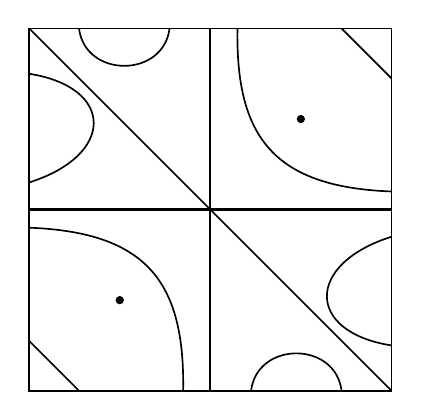
\begin{tikzpicture}[line width=0.6pt,scale=1.15]
  \draw (0,0) rectangle (4,4);
  \draw[line width=1.1pt] (0,2)--(4,2);
  \draw (2,0)--(2,4);
  \draw (0,4)--(4,0);
  \draw (0.55,4) .. controls (0.62,3.45) and (1.48,3.45) .. (1.55,4);
  \draw (0,3.5) .. controls (0.95,3.35) and (0.95,2.6) .. (0,2.3);
  \draw (0,1.8) .. controls (1.3,1.75) and (1.72,1.2) .. (1.7,0);
  \draw (0,0.55)--(0.55,0);
  \fill (1.0,1.0) circle (1.3pt);
  \draw (2.3,4) .. controls (2.28,2.8) and (2.7,2.25) .. (4,2.2);
  \draw (3.45,4)--(4,3.45);
  \fill (3.0,3.0) circle (1.3pt);
  \draw (3.45,0) .. controls (3.38,0.55) and (2.52,0.55) .. (2.45,0);
  \draw (4,0.5) .. controls (3.05,0.65) and (3.05,1.4) .. (4,1.7);
\end{tikzpicture}
\caption{\trTorus{}上一个具有三个\trCriticalPoint{}的函数的\trLevelSet}
\label{fig:monkey-saddle-torus}
\end{figure}

此外，在一个维数为 $n$ 的\trCompact\trConnected\trManifold{}上，构造一个具有 $n+1$ 个\trCriticalPoint{}的函数也是可能的。[76]~中发展了这样一套策略：先在\trManifold{}上构造一个\trMorseFunction，使其\trCriticalLevel{}集至多有 $n+1$ 个并且全都\trConnected{}（这是\trSmale{}的一个结果，参见~[53]），随后再在每个\trCriticalLevel{}集的邻域内修改这个函数，使得它在这个\trLevelSet{}内只有一个（\trDegenerate{}的）\trCriticalPoint。

\begin{example}\label{thm:euler-characteristic-sphere}
\trSphere{} $S^n$ 的\trEulerCharacteristic{}为
\[
\chi(S^n)=1+(-1)^n\text{，}
\]
也就是说，$n$ 为奇数时它为 $0$，$n$ 为偶数时它为 $2$。例如，维数为 2 的\trSphere{}的\trEulerCharacteristic{}就是 2。这还是那个\trEuler、还是那个 2、也还是那个\trAlternating{}和——正是“\trEuler{}多面体公式”里的那些：它说的乃是一个\trConnected{}多面体的面数 $F$、棱数 $E$ 与顶点数 $V$ 所满足的 $F-E+V=2$。
\end{example}

\begin{remark}\label{thm:euler-odd-dimension-zero}
无边界且维数为奇数的\trCompact\trManifold{}，其\trEulerCharacteristic{}为零：由\trPoincareDuality，\trAlternating{}和中各项两两相消。
\end{remark}

利用诸\trBettiNumber{} $\beta_k(V)=\dim HM_k(V;\ZZ/2)$，我们定义\trPoincarePolynomial
\[
P_V(t)=\sum_k\beta_k(V)\,t^k\text{。}
\]
例如，$P_{S^1}(t)=1+t$；更一般地，
\[
P_{S^n}(t)=1+t^n\text{。}
\]
此外，
\[
P_{\CP^n(\CC)}(t)=1+t^2+\dotsb+t^{2n}\text{，}
\]
而\footnote{译注：原书此处左端印作 $P_{\CP^2(\RR)}$，漏排自变量；同行 $P_{T^2}(t)$ 有之，疑系排印笔误；此处径补 $(t)$。——译者注}
\[
P_{T^2}(t)=1+2t+t^2\text{，}\qquad P_{\CP^2(\RR)}(t)=1+t+t^2\text{。}
\]
\trKunnethFormula{}立即给出关系式
\[
P_{V_1\times V_2}(t)=P_{V_1}(t)\,P_{V_2}(t)\text{。}
\]
记 $T^n=S^1\times\dotsb\times S^1$（$n$ 个因子），便可推出
\[
\beta_k(T^n)=\binom{n}{k}\text{。}
\]
特别地，应用\cref{thm:diffeomorphism-homology}，我们推出：只有当 $n=1$ 时，\trSphere{} $S^n$ 才与\trTorus{} $T^n$ \trDiffeomorphic。要得到这个结果，显然有比\trMorse{}理论更快的办法（比如说，\trSphere{}是\trSimplyConnected{}的，而\trTorus{}则不是）。

由此还可以得出（取 $t=-1$）
\[
\chi(V_1\times V_2)=\chi(V_1)\chi(V_2)\text{。}
\]

\begin{example}\label{thm:chi-s2-product}
我们求得 $\chi(S^2\times S^2)=4$。把 $S^2$ 上的\trHeightFunction{}与它自身相加，便得到 $S^2\times S^2$ 上的一个\trMorseFunction，它只有四个\trCriticalPoint：一个极小点、一个极大点以及两个\trIndex{}为 2 的\trCriticalPoint——这与我们的结果一致，因为 $1+2+1=4$。
\end{example}
